\section{Similarity-based Methods}

Similarity-based metrics are the simplest one in link prediction, in
which for each pair \(x\) and \(y\), a similarity score \(S(x, y)\) is
calculated. The score \(S(x, y)\) is based on the structural or node's
properties of the considered pair. The non-observed links (i.e.,
\(U - E^T\) ) are assigned scores according to their similarities.
\textbf{The pair of nodes having a higher score represents the predicted
    link between them}. The similarity measures between every pair \emph{can
    be calculated using several properties of the network}, one of which is
structural property. Scores based on this property can be grouped in
several categories like \textbf{local and global}, and so on.

\subsection{Local similarity indices}

Local indices are generally calculated using information about common
neighbors and node degree. These indices \textbf{consider immediate
    neighbors of a node}. The following are some examples of local
similarity indices with a description and method to calculate them:

\begin{itemize}
    \item \texttt{Common\ Neighbors\ (CN)}: In a given network or graph, the size
          of common neighbors for a given pair of nodes \(x\) and \(y\) is
          calculated as the size of the intersection of the two nodes
          neighborhoods ( \(\Gamma\) ). \[S(x, y) = |\Gamma(x) \cap \Gamma(y)|\]
          The likelihood of the existence of a link between x and y increases with
          the number of common neighbors between them.
    \item \texttt{Jaccard\ Coefficient}: This metric is similar to the Common
          Neighbors. Additionally, it normalizes the above score, as given below:
          \[S(x, y) = \frac{|\Gamma(x) \cap \Gamma(y)|}{|\Gamma(x) \cup \Gamma(y)|}\]
          The Jaccard coefficient is defined as the probability of selection of
          common neighbors of pairwise vertices from all the neighbors of either
          vertex. The pairwise Jaccard score increases with the number of common
          neighbors between the two vertices considered. Some researcher
          (\textbf{Liben-Nowell et al.}) demonstrated that this similarity metric
          \textbf{performs worse} as compared to Common Neighbors.
    \item \texttt{Adamic/Adar\ Index\ (AA)}: Adamic and Adar presented a metric to
          calculate a similarity score between two web pages based on shared
          features, which are further used in link prediction after some
          modification
          \[S(x, y) = \sum_{z \in \Gamma(x) \cap \Gamma(y)} \frac{1}{log k_z}\]
          where \(k_z\) is the degree of the node \(z\). It is clear from the
          equation that more weights are assigned to the common neighbors having
          smaller degrees. This is also intuitive in the real-world scenario, for
          example, a person with more number of friends spend less time/resource
          with an individual friend as compared to the less number of friends.
    \item \texttt{Preferential\ Attachment\ (PA)}: The idea of preferential
          attachment is applied to generate a growing scale-free network. The term
          \textbf{growing} represents the incremental nature of nodes over time in
          the network. The likelihood incrementing new connection associated with
          a node \(x\) is proportional to \(k_x\) , the degree of the node.
          Preferential attachment score between two nodes x and y can be computed
          as: \[S(x, y) = k_x k_y\] This index shows the worst performance on most
          networks. The \textbf{simplicity} (as it requires the least information
          for the score calculation) and the \textbf{computational time} of this
          metric are the main advantages. PA shows better results if larger degree
          nodes are densely connected, and lower degree nodes are rarely
          connected. In the above equation, summation can also be used instead of
          multiplication as an aggregate function.
    \item \texttt{Resource\ Allocation\ Index\ (RA)}: Consider two non-adjacent
          vertices \(x\) and \(y\). Suppose node \(x\) sends some resources to
          \(y\) through the common nodes of both \(x\) and \(y\) then the
          similarity between the two vertices is computed in terms of
          \textbf{resources sent} from \(x\) to \(y\). This is expressed
          mathematically as:
          \[S(x, y) = \sum_{z \in \Gamma(x) \cap \Gamma(y)} \frac{1}{k_z}\] The
          difference between \textbf{RA} and \textbf{AA} is that the RA index
          heavily penalizes to higher degree nodes compared to the AA index.
          Prediction results of these indices become almost the same for smaller
          average degree networks. This index shows good performance on
          heterogeneous networks with a high clustering coefficient, especially on
          transportation networks.
    \item \texttt{Cosine\ similarity\ or\ Salton\ Index\ (SI)}: This similarity
          index between two records (documents) is measured by calculating the
          Cosine of the angle between them. The metric is all about the
          orientation and not magnitude. The Cosine similarity can be computed as
          \[S(x, y) = \frac{|\Gamma(x) \cap \Gamma(y)|}{\sqrt{(k_x k_y)}}\] -
          \texttt{Sorensen\ Index}: It is very similar to the Jaccard index.
          \textbf{McCune et al.} show that it \textbf{is more robust than Jaccard
              against the outliers}.
          \[S(x, y) = \frac{2|\Gamma(x) \cap \Gamma(y)|}{k_X + k_y}\]
    \item \texttt{CAR-based\ Common\ Neighbor\ Index\ (CAR)}: CAR-based indices
          are presented based on the assumption that the link existence between
          two nodes is more likely if their common neighbors are members of a
          local community (local-community-paradigm (LCP) theory). In other words,
          the likelihood existence increases with the number of links among the
          common neighbors (local community links (LCLs)) of the seed node pair as
          described in the following figure.
          \[S(x, y) = CN(x, y) \text{ x } LCL(x, y) = CN(x, y) \text{ x } \sum_{z \in \Gamma(x) \cap \Gamma(y)} \frac{|\gamma(z)|}{2} \]
          where \(CN(x, y) = |\Gamma(x) ∩ \Gamma(y)|\) is number of common
          neighbors. \(LCL(x, y)\) refers to the number of local community links
          which are defined as the links among the common neighbors of seed nodes
          x and y. \(\gamma(z)\) is the subset of neighbors of node \(z\) that are
          also common neighbors of \(x\) and \(y\).

          \begin{figure}[H]
              \centering
              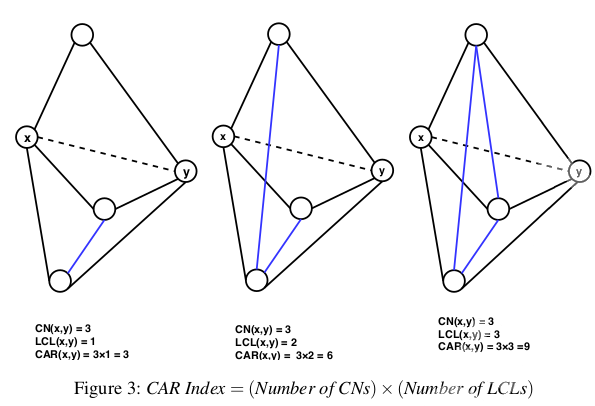
\includegraphics[width=8cm, keepaspectratio]{capitoli/methods/imgs/img3.png}
          \end{figure}
    \item \texttt{CAR-based\ Adamic/Adar\ Index\ (CAA)}: If \(LCL\) is considered
          as an accuracy enhancer, then the \(CAA\) index is obtained by
          incorporating the \(LCL\) theory to the well known AA index and
          mathematically expressed by the equation given below.
          \[S(x, y) = \sum_{z \in \Gamma(x) \cap \Gamma(y)} \frac{|\gamma(z)|}{\log_2(k_z)} \]
    \item \texttt{CAR-based\ Resource\ Allocation\ Index\ (CRA)}: Is a general
          application of the LCL theory to other indices and generate the CRA
          index by incorporating this concept into the existing RA index of the
          literature. Mathematically, the CRA can be expressed as
          \[S(x, y) = \sum_{z \in \Gamma(x) \cap \Gamma(y)} \frac{|\gamma(z)|}{k_z}\]
    \item \texttt{CAR-based\ Preferential\ Attachment\ Index\ (CPA)}: This is
          the preferential attachment index based on the CAR index. CPA is
          obtained by incorporating the LCL theory to the original PA method and
          expressed mathematically by
          \[S(x, y) = e_x e_y + e_x CAR(x, y) + e_y CAR(x, y) + CAR(x, y)^2\]
          where \(e_x\) is the number of neighbors of \(x\) not shared by \(y\)
          and \(CAR(x, y)\) is the similarity score of the node pair \(x\) and
          \(y\) using CAR index. CAR-based methods listed above show the best
          performance on LCP networks. The LCP networks are related to dynamic and
          heterogeneous systems and facilitate network evolution of social and
          biological networks.
    \item \texttt{Hub\ Promoted\ Index\ (HPI)}: This
          similarity index promotes the formation of links between the sparsely
          connected nodes and hubs. It also tries to prevent links formation
          between the hub nodes. This similarity metric can be expressed
          mathematically as
          \[S(x, y) = \frac{|\Gamma(x) \cap \Gamma(y)|}{min(k_x, k_y)}\]
    \item \texttt{Hub\ Depressed\ Index\ (HDI)}: This index is the same as the
          previous one but with the opposite goal as it avoids the formation of
          links between hubs and low degree nodes in the networks. The Hub
          depressed index promotes the links evolution between the hubs as well as
          the low degree nodes. The mathematical expression for this index is
          given below.
          \[S(x, y) = \frac{|\Gamma(x) \cap \Gamma(y)|}{max(k_x, k_y)}\]
    \item \texttt{Local\ Naive\ Bayes-based\ Common\ Neighbors\ (LNBCN)}: The
          above similarity indices are somehow based on common neighbors of the
          node pair where each of the which are equally weighted. This method is
          based on the Naive Bayes theory and arguments that different common
          neighbors play different role in the network and hence contributes
          differently to the score function computed for non-observed node pairs
          \[S(x, y) = \sum_{z \in \Gamma(x) \cap \Gamma(y)} [log(\frac{C(z)}{1 - C(z)}) + log(\frac{1 - \rho}{\rho})]\]
          where \(C(z)\) is node clustering coefficient and \(\rho\) is the
          network density expressed as \[\rho = \frac{|E|}{n(n-1)/2}\]
    \item \texttt{Leicht-Holme-Newman\ Local\ Index\ (LHNL)}: The logic below this
          index is that two vertices are similar to each other if their
          corresponding neighbors are self-similar to themselves. This score is
          defined by the ratio of the path of length two that exits between two
          vertices and the expected path of the same length between them.
          \[S(x, y) = \frac{|\Gamma(x) \cap \Gamma(y)|}{k_x k_y}\]
    \item \texttt{Node\ Clustering\ Coefficient\ (CCLP)}: This index is also based
          on the clustering coefficient property of the network in which the
          clustering coefficients of all the common neighbors of a seed node pair
          are computed and summed to find the final similarity score of the pair.
          Mathematically \[S(x, y) = \sum_{z \in \Gamma(x) \cap \Gamma(y)} C(z)\]
          where \[C(z) = \frac{t(z)}{k_z(k_z - 1)}\] is clustering coefficient of
          the node \(z\) and \(t(z)\) is the total triangles passing through the
          node \(z\).
    \item \texttt{Node\ and\ Link\ Clustering\ coefficient\ (NLC)}:
          This similarity index is based on the basic topological feature of a
          network called ''\emph{Clustering Coefficient}''. The clustering
          coefficients of both nodes and links are incorporated to compute the
          similarity score.
          \[S(x, y) = \sum_{z \in \Gamma(x) \cap \Gamma(y)} \frac{|\Gamma(x) \cap \Gamma(z)|}{k_z -1} \text{ x }C(z) + \frac{|\Gamma(y) \cap \Gamma(z)|}{k_z -1} \text{ x }C(z)\]

\end{itemize}

\subsection{Global similarity indices}

Global indices are computed using entire topological information of a
network. The computational complexities of such methods are higher and
seem to be infeasible for large networks.

\begin{itemize}
    \item \texttt{Katz\ Index}: This
          index can be considered as a variant of the shortest path metric. It
          directly aggregates over all the paths between x and y and dumps
          exponentially for longer paths to penalize them. It can be expressed
          mathematically as:
          \[S(x, y) = \sum_{l = 1}^{\infty}\beta^l|paths_{x, y}^{<l>}| = \sum_{l = 1}^{\infty}\beta^l(A)^l_{x, y}\]
          where, \(paths_{x, y}^{<l>}\) is considered as the set of total \(l\)
          length paths between \(x\) and \(y\), \(\beta\) is a damping factor that
          controls the path weights and A is the adjacency matrix. For the
          convergence of above equation, \[\beta < \frac{1}{\lambda_1} \] where
          \(\lambda_1\) is the maximum eigenvalue of the matrix A. If 1 is added
          to each element of the diagonal of the resulting similarity matrix S,
          this expression can be written in matrix terms as \[S = \beta AS + I\]
          where \(I\) is the identity matrix of the proper dimension. The
          similarity between all pairs of nodes can be directly computed using the
          closed-form by rearranging for \(S\) in the previous expression and
          subtracting the previously added 1 to the elements in the diagonal. Katz
          score for each pair of nodes in the network is calculated by finding the
          similarity matrix as \[S = (I - \beta A)^{- 1} - I\] The computational
          complexity of the given metric is high, and it can be roughly estimated
          to be cubic complexity which is not feasible for a large network.
    \item \texttt{Random\ Walk\ with\ Restart\ (RWR)}: Let \(\alpha\) be a
          probability that a random walker iteratively moves to an arbitrary
          neighbor and returns to the same starting vertex with probability
          \((1 - \alpha)\). Consider \(q_{xy}\) to be the probability that a
          random walker who starts walking from vertex \(x\) and located at the
          vertex \(y\) in steady-state. Now, this probability of walker to reach
          the vertex \(y\) is expressed mathematically as
          \[\overrightarrow{q_x} = \alpha P^T \overrightarrow{q_x} + (1-\alpha) \overrightarrow{e_x}\]
          where \(\overrightarrow{e_x}\) is the seed vector of length \(|V|\)
          (i.e., the total number of vertices in the graph). This vector consists
          of zeros for all components except the elements \(x\) itself. The
          transition matrix \(P\) can be expressed as
          \[\overrightarrow{q_x} = (1-\alpha)(I - \alpha P^T)^{-1} \overrightarrow{e_x}\]
          Since this similarity is not symmetric, the final score between the node
          pair (x, y) can be computed as \[S(x, y) = q_{xy} + q_{yx}\] It is clear
          from the above equation that matrix inversion is required to solve,
          which is quite expensive and prohibitive for large networks.
    \item \texttt{Shortest\ Path}: The inverse relation between the similarity and
          length of the shortest path is captured by the following mathematical
          equation given below. \[S(x, y) = -|d(x, y)|\] where Dijkstra algorithm
          is applied to efficiently compute the shortest path d(x, y) between the
          node pair (x, y). The prediction accuracy of this index is low compared
          to most local indices.
    \item \texttt{Leicht-Holme-Newman\ Global\ Index\ (LHNG)}: This global index
          is based on the principle that two nodes are similar if either of them
          has an immediate neighbor, which is similar to the other node. This is a
          recursive definition of similarity where a termination condition is
          needed. The termination condition is introduced in terms of
          self-similarity, i.e., a node is similar to itself. Thus, the similarity
          score equation consists of two terms: first, the neighbor similarity,
          and the second, self-similarity, as given below.
          \[S(x, y) = \phi  \sum_z A_{x, z} S_{z, y} + \psi \delta_{x, y}\] Here,
          the first term is neighborhood similarity and the second term is
          self-similarity. \(\psi\) and \(\phi\) are free parameters that make a
          balance between these two terms. When the free parameter \(\psi\) = 1,
          this index resembles to the Katz index.
    \item \texttt{Cosine\ based\ on\ L+\ (Cos+)}: Laplacian matrix is extensively
          used as an alternative representation of graphs in spectral graph
          theory. This matrix can be defined as \(L = D - A\), where, \(D\) is the
          diagonal matrix consisting of the degrees of each node of the matrix and
          \(A\) is the adjacency matrix of the graph. The pseudo-inverse of the
          matrix defined by Moore-Penrose is represented as \(L^+\) and each entry
          of this matrix is used to represent the similarity score between the two
          corresponding nodes. The most common way to compute this pseudo-inverse
          is by computing the \textbf{singular value decomposition (SVD)} of the
          Laplacian matrix [$(L = U \Sigma V^{}T)$, where \(U\) and \(V\)
                  are left and right singular vectors of \(SVD\)] as follows
          \[L^+ = V \Sigma^+ U^T\] \(\Sigma^+\) is obtained by taking the inverse
          of each nonzero element of the \(\Sigma\). Further, the similarity
          between two nodes \(x\) and \(y\) can be computed using any inner
          product measure such as Cosine similarity given as
          \[S(x, y) = \frac{L_{x, y}^+}{\sqrt{L_{x, x}^+ L_{y, y}^+}}\]
    \item \texttt{Average\ Commute\ Time\ (ACT)}: This index is based on the
          random walk concept. A random walk is a Markov chain which describes the
          movements of a walker. It defined as the average number of
          movements/steps required by a random walker to reach the destination
          node \(y\), and come back to the starting node \(x\). If \(m(x, y)\) be
          the number of steps required by the walker to reach \(y\) from \(x\),
          then the following expression captures this concept.
          \[n(x, y) = |E| (l_{xx}^+ + l_{yy}^+ - 2l_{xy}^+) \] where \(l_{xy}^+\)
          denotes the \((x, y)\) entry of the matrix \(L^+\) . Pseudo-inverse of
          the Laplacian, \(L^+\) can be computed as
          \[L^+ = (L - \frac{ee^T}{n})^{-1} + \frac{ee^T}{n}\] where \(e\) is a
          column vector consisting of 1's. Smaller value of this equation will
          represent higher similarity. The final expression is the following
          \[S(x, y) = \frac{1}{l_{xx}^+ + l_{yy}^+ - 2l_{xy}^+}\]
    \item \texttt{Normalized\ Average\ Commute\ Time\ (NACT)}: This is a variant
          of ACT that takes into account node degrees. For a high degree node
          (hub) \(y\), \(m(x, y)\) is usually small regardless of \(x\), the
          similarity measure is normalized with stationary distribution \(\pi\) of
          the Markov chain describing random walker on the graph. This normalized
          measure can be computed with the following equation
          \[S(x, y) = \frac{1}{(m(x, y)\pi_y + m(y, x)\pi_x)}\]
    \item \texttt{Matrix\ Forest\ Index\ (MF)}: his index is based on the concept
          of spanning tree which is defined as the subgraph that spans total nodes
          without forming any cycle. The spanning tree may contain total or less
          number of links as compared to the original graph. Chebotarev and Shamis
          proposed a theorem called matrix-forest theorem which states that the
          number of spanning tree in a graph is equal to the co-factor of any
          entry of Laplacian matrix of the graph. Here, the term forest represents
          the union of all rooted disjoint spanning trees. The similarity between
          two nodes \(x\) and \(y\) can be computed with the equation given below
          \[S = (I + L)^{-1}\] where \((I + L)\_{(x,y)}\) is the number of
          spanning rooted forests ( \(x\) as root ) consisting of both the nodes
          \(x\) and \(y\). Moreover, this quantity is equal to the co-factor of
          \((I + L)_{(x,y)}\) .
    \item \texttt{SimRank}: This is a measure of
          structural context similarity and shows object-to-object relationships.
          It is not domain-specific and recommends to apply in directed or mixed
          networks. The basic assumption of this measure is that two objects are
          similar if they are related to similar objects. SimRank computes how
          soon two random walkers meet each other, starting from two different
          positions. This measure can be represented in matrix form as
          \[S(x,y) = \alpha W^T SW + (1 - \alpha)I\] where, \(\alpha \in (0, 1)\)
          is a constant. \(W\) is the transformation matrix and computed by
          normalizing each column of adjacency matrix \(A\) as
          \[
              W_{ij} = \frac{a_{ij}}{\sum_{k=1}^{n}}
          \]
          The computational complexity
          of this measure is high for a large network, and to reduce its time, the
          authors suggest pruning recursive branches.
    \item \texttt{Rooted\ Pagerank\ (RPR)}: The idea of PageRank was originally
          proposed to rank the web pages based on the importance of those pages.
          The algorithm is based on the assumption that a random walker randomly
          goes to a web page with probability \(\alpha\) and follows hyper-link
          embedded in the page with probability \((1 - \alpha)\). Chung et
          al.~used this concept incorporated with a random walk in link prediction
          framework. The importance of web pages, in a random walk, can be
          replaced by stationary distribution. The similarity between two vertices
          \(x\) and \(y\) can be measured by the stationary probability of \(y\)
          from \(x\) in a random walk where the walker moves to an arbitrary
          neighboring vertex with probability \(\alpha\) and returns to \(x\) with
          probability \((1 - \alpha)\). Mathematically, this score can be computed
          for all pair of vertices as
          \[RPR = (1 - \alpha)(I - \alpha \hat{N})^{-1}\] where
          \(\hat{N} = D^{-1} A\) is the normalized adjacency matrix with the
          diagonal degree matrix \(D[i, i] = \sum_j A[i, j]\).
\end{itemize}

\subsection{Quasi-local indices}

Quasi-local indices have been introduced as a trade-off between local
and global approaches or performance and complexity. These metrics are
as efficient to compute as local indices. Some of these indices extract
the entire topological information of the network. The time complexities
of these indices are still below compared to the global approaches.

\begin{itemize}
    \item \texttt{Local\ Path\ Index\ (LP)}: This metric has the intent to furnish
          a good trade-off between accuracy and computational complexity. The
          metric is expressed mathematically as \[S^{LP} = A^2 + \epsilon A^3\]
          where $\epsilon$ represents a free parameter. Clearly, the measurement
          converges to common neighbor when \(\epsilon = 0\). If there is no
          direct connection between \(x\) and \(y\), \((A^3)_{xy}\) is equated to
          the total different paths of length 3 between \(x\) and \(y\). The index
          can also be expanded to generalized form
          \[S^{LP} = A^2 + \epsilon A^3 + \epsilon^2 A^4 + ... + \epsilon^{(n−2)} A^n\]
          where \(n\) is the maximal order. Computing this index becomes more
          complicated with the increasing value of \(n\). The LP index outperforms
          the proximity-based indices, such as RA, AA, and CN.
    \item \texttt{Path\ of\ Length\ 3\ (L3)}: Georg Simmel, a German sociologist,
          first coined the concept ``triadic closure'' and made popular by Mark
          Granovetter in his work ``\emph{The Strength of Weak Ties}''. The
          authors proposed a similarity index in protein-protein interaction (PPI)
          network, called \textbf{\emph{path of length 3 (or L3)}} published in
          the Nature Communication. They experimentally show that the triadic
          closure principle (TCP) does not work well with PPI networks. They
          showed the paradoxical behavior of the TCP (i.e., the path of length 2),
          which does not follow the structural and evolutionary mechanism that
          governs protein interaction. The TCP predicts well to the interaction of
          self-interaction proteins (SIPs), which are very small (4\%) in PPI
          networks and fails in prediction between SIP and non SIP that amounts to
          96\%. They showed that the L3 index performs well in such conditions and
          give mathematical expression to compute this index as
          \[S(x, y) = \sum \frac{a_{x,u} a_{u,v} a_{v,y}}{k_u k_v}\]
    \item \texttt{Similarity\ based\ on\ Local\ Random\ Walk\ and\ Superposed\ Random\ Walk\ (LRW\ and\ SRW)}:
          This metric propose a new similarity measures by exploiting the random
          walk concept on graphs with limited walk steps. They defined node
          similarity based on random walks of lower computational complexity
          compared to the other random walk based methods. Given a random walker,
          starting from the node \(x\), the probability of reaching the random
          walker to the node \(y\) in \(t\) steps is
          \[\overrightarrow{\pi}\_x(t) = P^T \overrightarrow{\pi}\_x(t-1)\] where
          \(\overrightarrow{\pi}\_x(0)\) is a column vector with \(x^{th}\)
          element as 1 while others are 0's and \(P^T\) is the transpose of the
          transition probability matrix \(P\). \(P_{xy}\) entry of this matrix
          defines the probability of a random walker at node \(x\) will move to
          the next node \(y\). It is expressed as \(P_{xy} = \frac{a_{kx}}{k_x}\)
          , where \(a_{xy}\) is 1 when there is a link between \(x\) and \(y\) and
          0, otherwise. The authors computed the similarity score ( \(LRW\) )
          between two nodes based on the above concept as
          \[S^{LRW}(x, y) = \frac{k_x}{2|E|}\pi_{xy}(t) + \frac{k_y}{2|E|}\pi_{xy}(t)\]
          This similarity measure focus on only few steps covered by the random
          walker (hence quasi-local) and not the stationary state compared to
          other approaches. Random walk based methods suffer from the situation
          where a random walker moves far away with a certain probability from the
          target node whether the target node is closer or not. This is an obvious
          problem in social networks that show a high clustering index i.e.,
          clustering property of the social networks. This degrades the similarity
          score between the two nodes and results in low prediction accuracy. One
          way to counter this problem is that continuously release the walkers at
          the starting point, which results in a higher similarity between the
          target node and the nearby nodes. By superposing the contribution of
          each walker (walkers move independently), SRW is expressed as
          \[S^{SRW} (x, y) (t) = \sum_{l=1}^{t} S^{LRW} (l)\]
\end{itemize}

\subsection{Some Remarks}

Similarity-based approaches mostly focus on the structural properties of
the networks to compute the similarity score. \textbf{\emph{Local
        approaches}} consider, in general, neighborhood information (direct
neighbors or neighbors of neighbor), which take less time for
computation. This is the property that makes the local approaches
feasible for massive real-world network datasets. \textbf{\emph{Global
        approaches}} consider the entire structural information of the network;
that is why time required to capture this information is more than local
and quasi-local approaches. Also, sometimes, entire topological
information may not be available at the time of computation, especially
in a decentralized environment. So, parallelization over the global
approaches may not possible or very complex compared to the local and
quasi-local approaches. The performance or prediction accuracy of these
approaches (i.e., global approaches) is better compared to local and
quasi-local. \textbf{\emph{Quasi-local approaches}} extract more
structural information than local and somehow less information compared
to the global.

